\section{Results}
\subsection{\fred as a Teaching Aid}

\fred (v0.0.3)\cite{stephen_thompson_2020_3946090} was used at our Medical Summer School in 2020 with a cohort of 5 students. Informal feedback indicated that it had improved their
understanding
of fiducial based registration. \fred also forms part of the \gls{BARD} which 
was a finalist at the MICCAI 2020 educational challenge 
\footnote{\href{https://miccai-sb.github.io/materials.html}{https://miccai-sb.github.io/materials.html}}. 

\subsection{Extension to Anisotropic Errors}
We simulated an anisotropic independent \gls{FLE}, with \gls{FLE} in the x 
direction being 3 times that in the y and z, as described in Section \ref{sec:anis_method}.
Errors were scaled so that the 
expected absolute value of the \gls{FLE} was the same as for the isotropic case. 
\fred was then used to perform at least 200 simulated registrations, the results of
which are shown in Fig. \ref{fig:anis_error}. 

\begin{figure}
	\begin{center}
			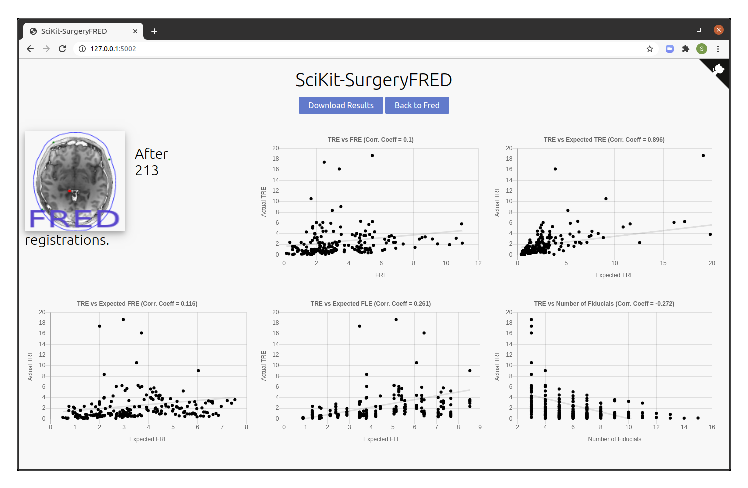
\includegraphics[width=0.9\linewidth]{images/anisitropic_error.eps}
		\caption{\label{fig:anis_error}Results of over 200 registrations using an anisotropic model of {FLE}}
	\end{center}
\end{figure}

It was apparent when performing the registrations that the majority of target 
registration error was in the x direction. However this is not communicated in the 
statistics of Figure \ref{fig:anis_error}. It would be an interesting extension 
exercise to use \fred to explore ways of communicating anisotropic errors during 
treatment.

\subsection{Addition of Systematic Errors}
We added a systematic \gls{FLE} as an isotropic uniform random variable, in the range
-0.5 to 0.5, as described in Section \ref{sec:sys_method}. This error will be applied to all fiducial markers for a 
given registration. We performed at least 200 simulated registrations using \fredns, the results of which are shown in Fig. \ref{fig:sys_error}.
\begin{figure}
	\begin{center}
			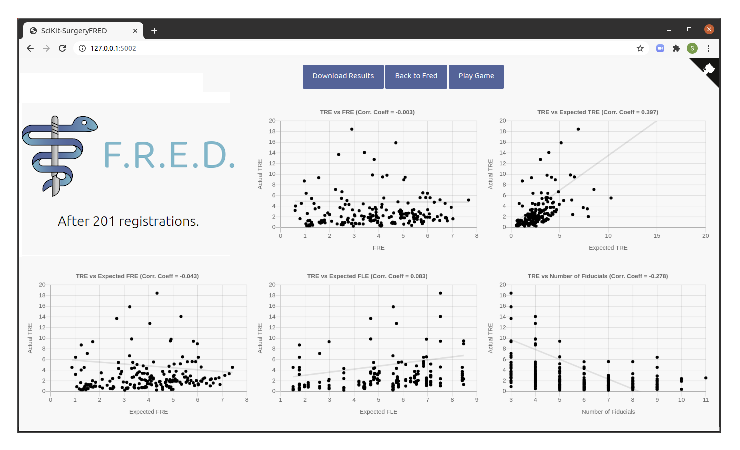
\includegraphics[width=0.9\linewidth]{images/systematic_error.eps}
			\caption{\label{fig:sys_error}Results of over 200 registrations with systematic error.}
	\end{center}
\end{figure}

It is noticeable that average \gls{TRE}s are higher than in cases where there is no
systematic error, while \gls{FRE} remains similar. This is as expected as \gls{FRE} will 
not account for systematic errors. This is a useful demonstration of this effect, though 
it might be more instructive to implement systematic errors in the game based method, see
Section \ref{sec:game_method}, to investigate the likely clinical impact of these
systematic errors.

\subsection{Statistical Significance}
As discussed in Section \ref{sec:methods} it is useful to perform tests of 
statistical significance on \fredns's registration results. 
We used the function \href{https://docs.scipy.org/doc/scipy/reference/generated/scipy.stats.linregress.html}{stats.linregress} from {SciPy}\cite{2020SciPy-NMeth} to
perform a Wald Test against the null hypothesis that the slope is zero. For the
results shown in Figures \ref{fig:correlation}, \ref{fig:anis_error}, 
and \ref{fig:sys_error} there was no significant
relationship between actual \gls{TRE} and either actual or expected \gls{FRE}. There was
a significant relationship between actual \gls{TRE} and the expected \gls{TRE}. All
of these results are as expected.

Tests against the expected value of \gls{FLE} and the number of fiducial markers are
more problematic, as they are not continuous variables, which should be apparent 
when looking at the results charts. The reason for this is obvious for the number
of fiducial markers. The expected value of \gls{FLE} is clustered into groups as this
is only set once for a given target, however the registration for this target 
will be repeated each time a new fiducial marker is added beyond the minimum of 3. Hence 
if the user adds a total of 10 fiducial markers, this will create 8 registration 
results all with different \gls{TRE} and \gls{FRE}, but with a single value of 
expected \gls{FLE}.


\subsection{\fred for Research}
The results of the game based usability study described in Section \ref{sec:game_method}
are shown in 
Figure \ref{fig:usability}. As expected scores are 
highest when the actual \gls{TRE} is known. Interestingly it appears that when told only the expected value of the \gls{FLE} the students
tended to under treat the target more, resulting in lower overall scores. 


\begin{figure}
        \begin{center}
        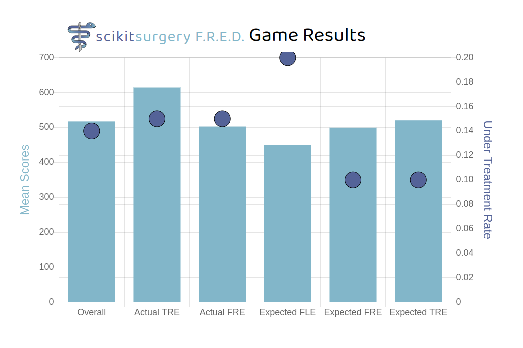
\includegraphics[width=0.5\linewidth]{usability.eps}
                \caption{\label{fig:usability}Average scores and treatment failure rates for the game based usability study.}
	\end{center}
\end{figure}

The statistical significance of the results was tested using a two sided T-test implemented
in {SciPy}'s\cite{2020SciPy-NMeth} \href{https://docs.scipy.org/doc/scipy/reference/generated/scipy.stats.ttest_ind.html}{stats.ttest{\textunderscore}ind} function.
Using a p-value of 0.05 none of the results were statistically significant. 
Currently there are only 100 data points (20 for each category), so this is not 
surprising. 


